\pagebreak
\section{Architectural Design}
 
\subsection{High level components}
In this section we are going to introduce the architecture that will be used to develop
the application. We based our decisions upon the requirements described in the RAS Document 
and we choose three principles as the foundations of our structure: 
\begin{itemize}
    \item \textbf{Client-server} model.
    \item \textbf{RESTful} API.
    \item \textbf{Microservices} approach.
\end{itemize}

\subsubsection{Client-Server}
The client-server aspect of our application can be seen in Figure~\ref{fig:h_l_comp}.
There we focus on the "physical" representation of our application. By saying physical we mean that
every component depicted there will reside on separate machines (or is an external service).
To be precise, we should have added another component between clients and
application server which is the reverse proxy/web server. The reason why we preferred to
omit it is that, at this stage, we want to address only the aspects that are relevant to the
application development and that layer can be considered transparent with respect to the application.
The application does not have to deal with it explicitly.
Of course this will not be the same in a context of deployment.
The interaction between client and server will be the usual one when dealing with web/mobile
applications. Our client will make the initial request and the server will send back the
information. In out case, such informations will be received as an XML or JSON document.

\subsubsection{RESTful API}
For the design of the API we decided to rely upon the REST principles. The reasons that moved
this decision are diverse. To begin with, we decided that a generic API was better fitting
in our context that is composed of different clients (web application, and different mobile
clients). This way, we can serve a single format of document as respond containing all the 
requested data and then the client can build the user interface using the most suitable
technologies according to the specific case.
Secondly, REST principles, when followed correctly, concur to gain desirable non-functional
features, such as performance, scalability, simplicity and modifiability.
Finally, messages exchanged in REST APIs are often self-descriptive and this is beneficial
for the ease of development of web and mobile applications.

\subsubsection{Microservices}
Figure~\ref{fig:i_h_l_comp} is a high level overview of the application internals stripped from all
the external components. We are going to describe its architecture further in this document
but we wanted nonetheless to give an initial idea.
The internal structure of the application is going to be a service oriented architecture.
Upon receiving a new request, the router (our entry point) will produce a new message,
that will be dispatched to all the required services. The response to this message will
be rendered and sent back to the client.
The reason why we choose microservices is that they allow us to separate the code in
atomic components, each of them dealing with a single responsibility.
Furthermore, using queues to dispatch messages, ensure that our internal communications
are asynchronous and non blocking.

\begin{sidewaysfigure}
\centering
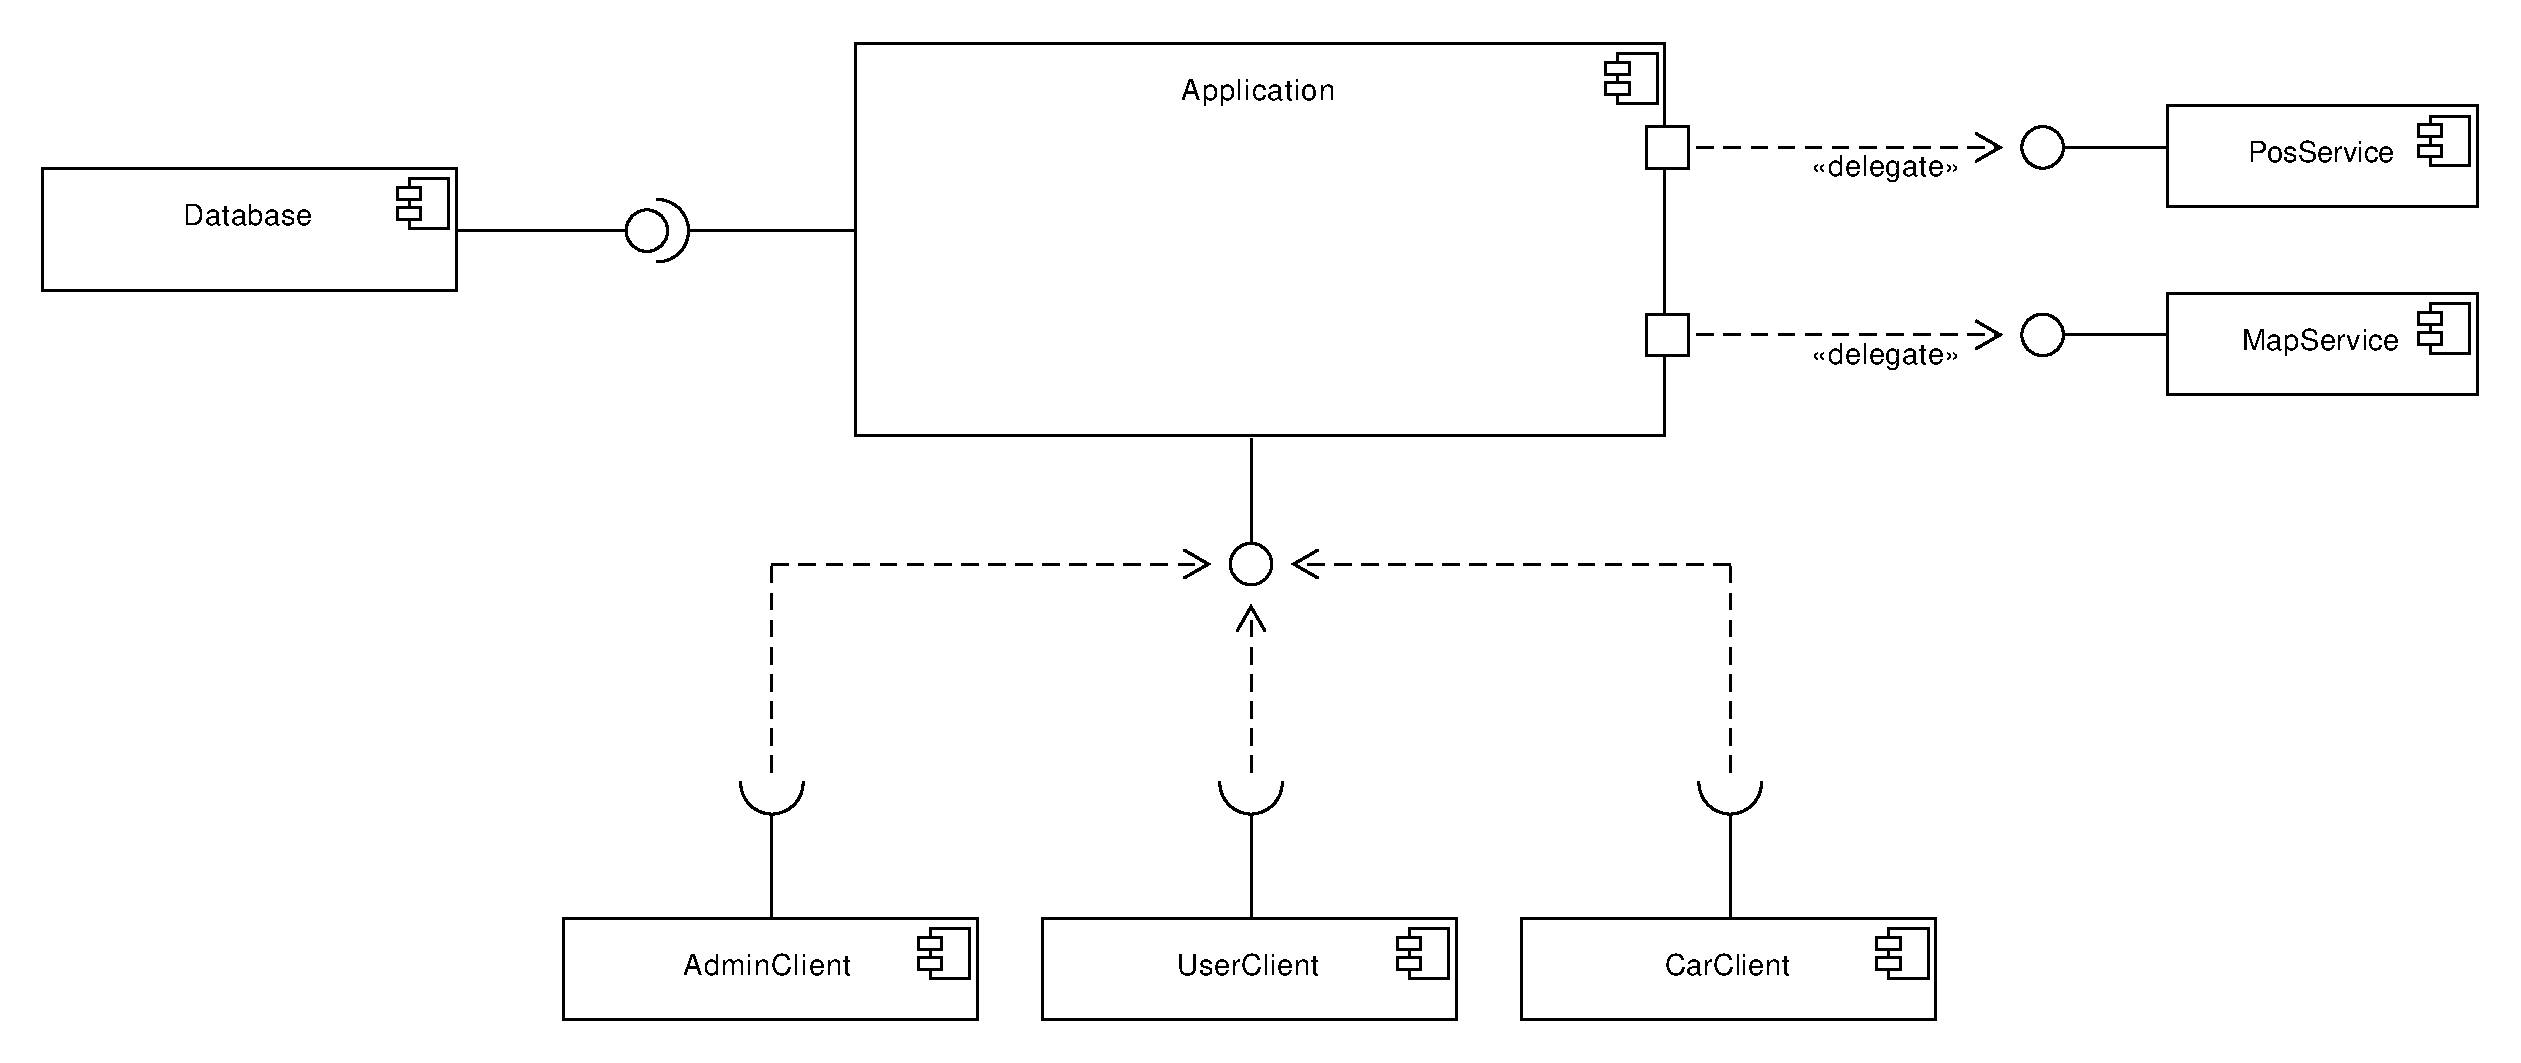
\includegraphics[width=\textwidth]{high_level_components}
\caption{Component view: High Level Architecture}
\label{fig:h_l_comp}
\end{sidewaysfigure}

\begin{sidewaysfigure}
\centering
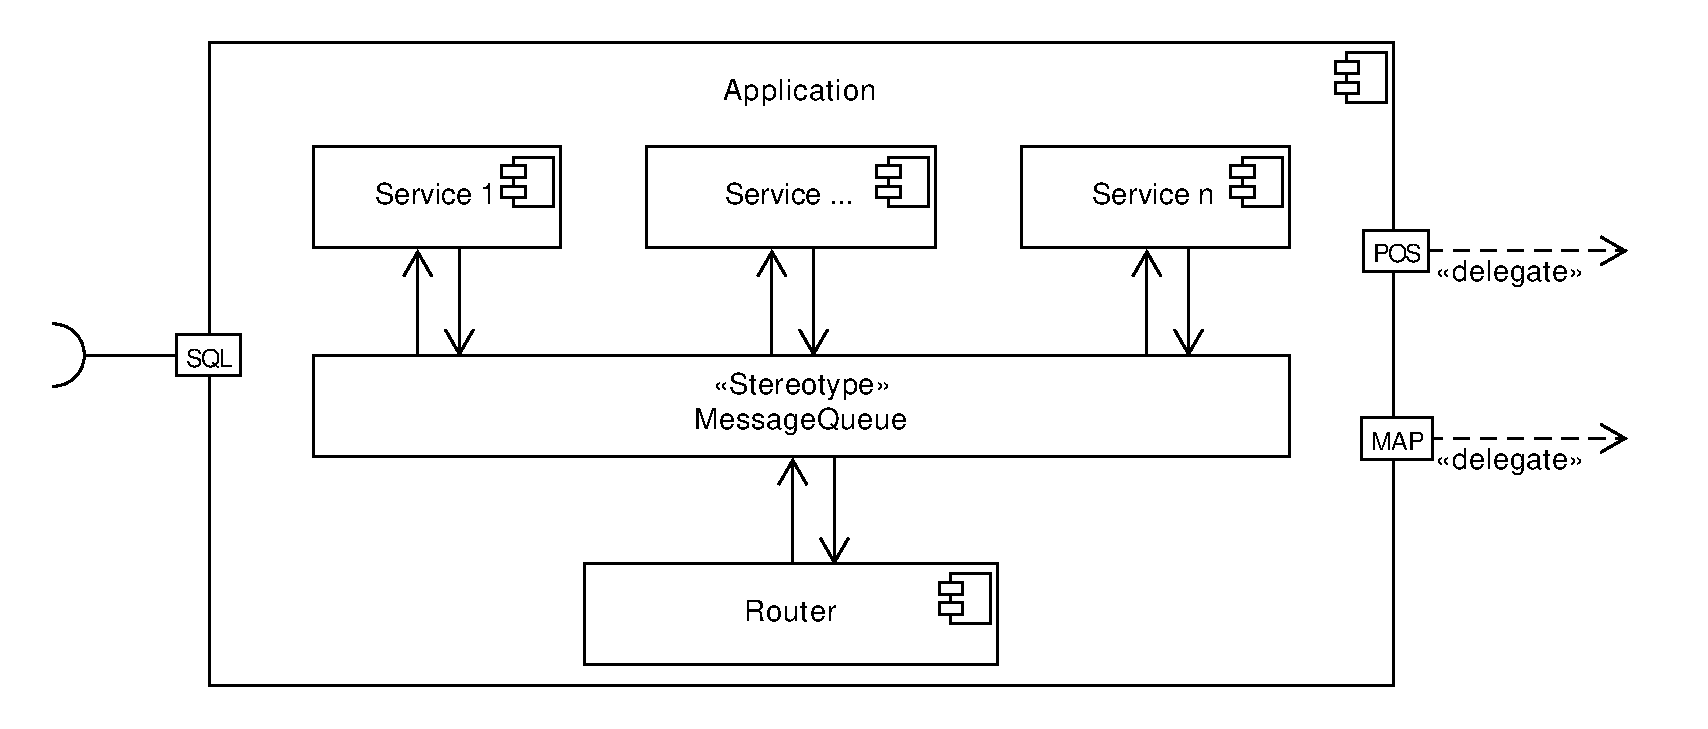
\includegraphics[width=\textwidth]{internal_high_level_components}
\caption{Component view: Internal High Level Architecture}
\label{fig:i_h_l_comp}
\end{sidewaysfigure}

\pagebreak
\subsection{Low level components}
In this section we are going to describe further the internal configuration of our server
application. After giving a general overview, we will analyze each component separately.
As we anticipated in the previous section, the application is going to follow the microservices
architecture internally with some functions delegated to external services or components.
We will start by describing the latter and then we will move on to the internal ones.
To do so we will use Figure~\ref{fig:i_l_l_comp} as a reference.
In that diagram you can see a more detailed example of what we have already seen
in Figure~\ref{fig:i_h_l_comp}.

\subsubsection{Map API}
Starting from the latter, we assume that all functions related to the map (path finding,
distance calculation, map representation, etc) will be delegated to the Google Maps API.
All the classes that are going to use that API will provide an additional interface if they 
need to expose some functionalities to the other components.
\subsubsection{POS API}
The other aspect that we are not going to develop internally is the Payment Service (POS).
In this case we are going to use the simple an powerful Stripe service that have been chosen
for its ease of use and of integration.
\subsubsection{Database}
Finally, the last component that will not be part of the application in a strict way is the database.
It won't be an entirely external service since we are going to host and mange it in our infrastructure,
but it's still something our application will user through its dedicated API. Regarding the
database we will use the solid and well tested PostgreSQL relational database.

\begin{sidewaysfigure}
\centering
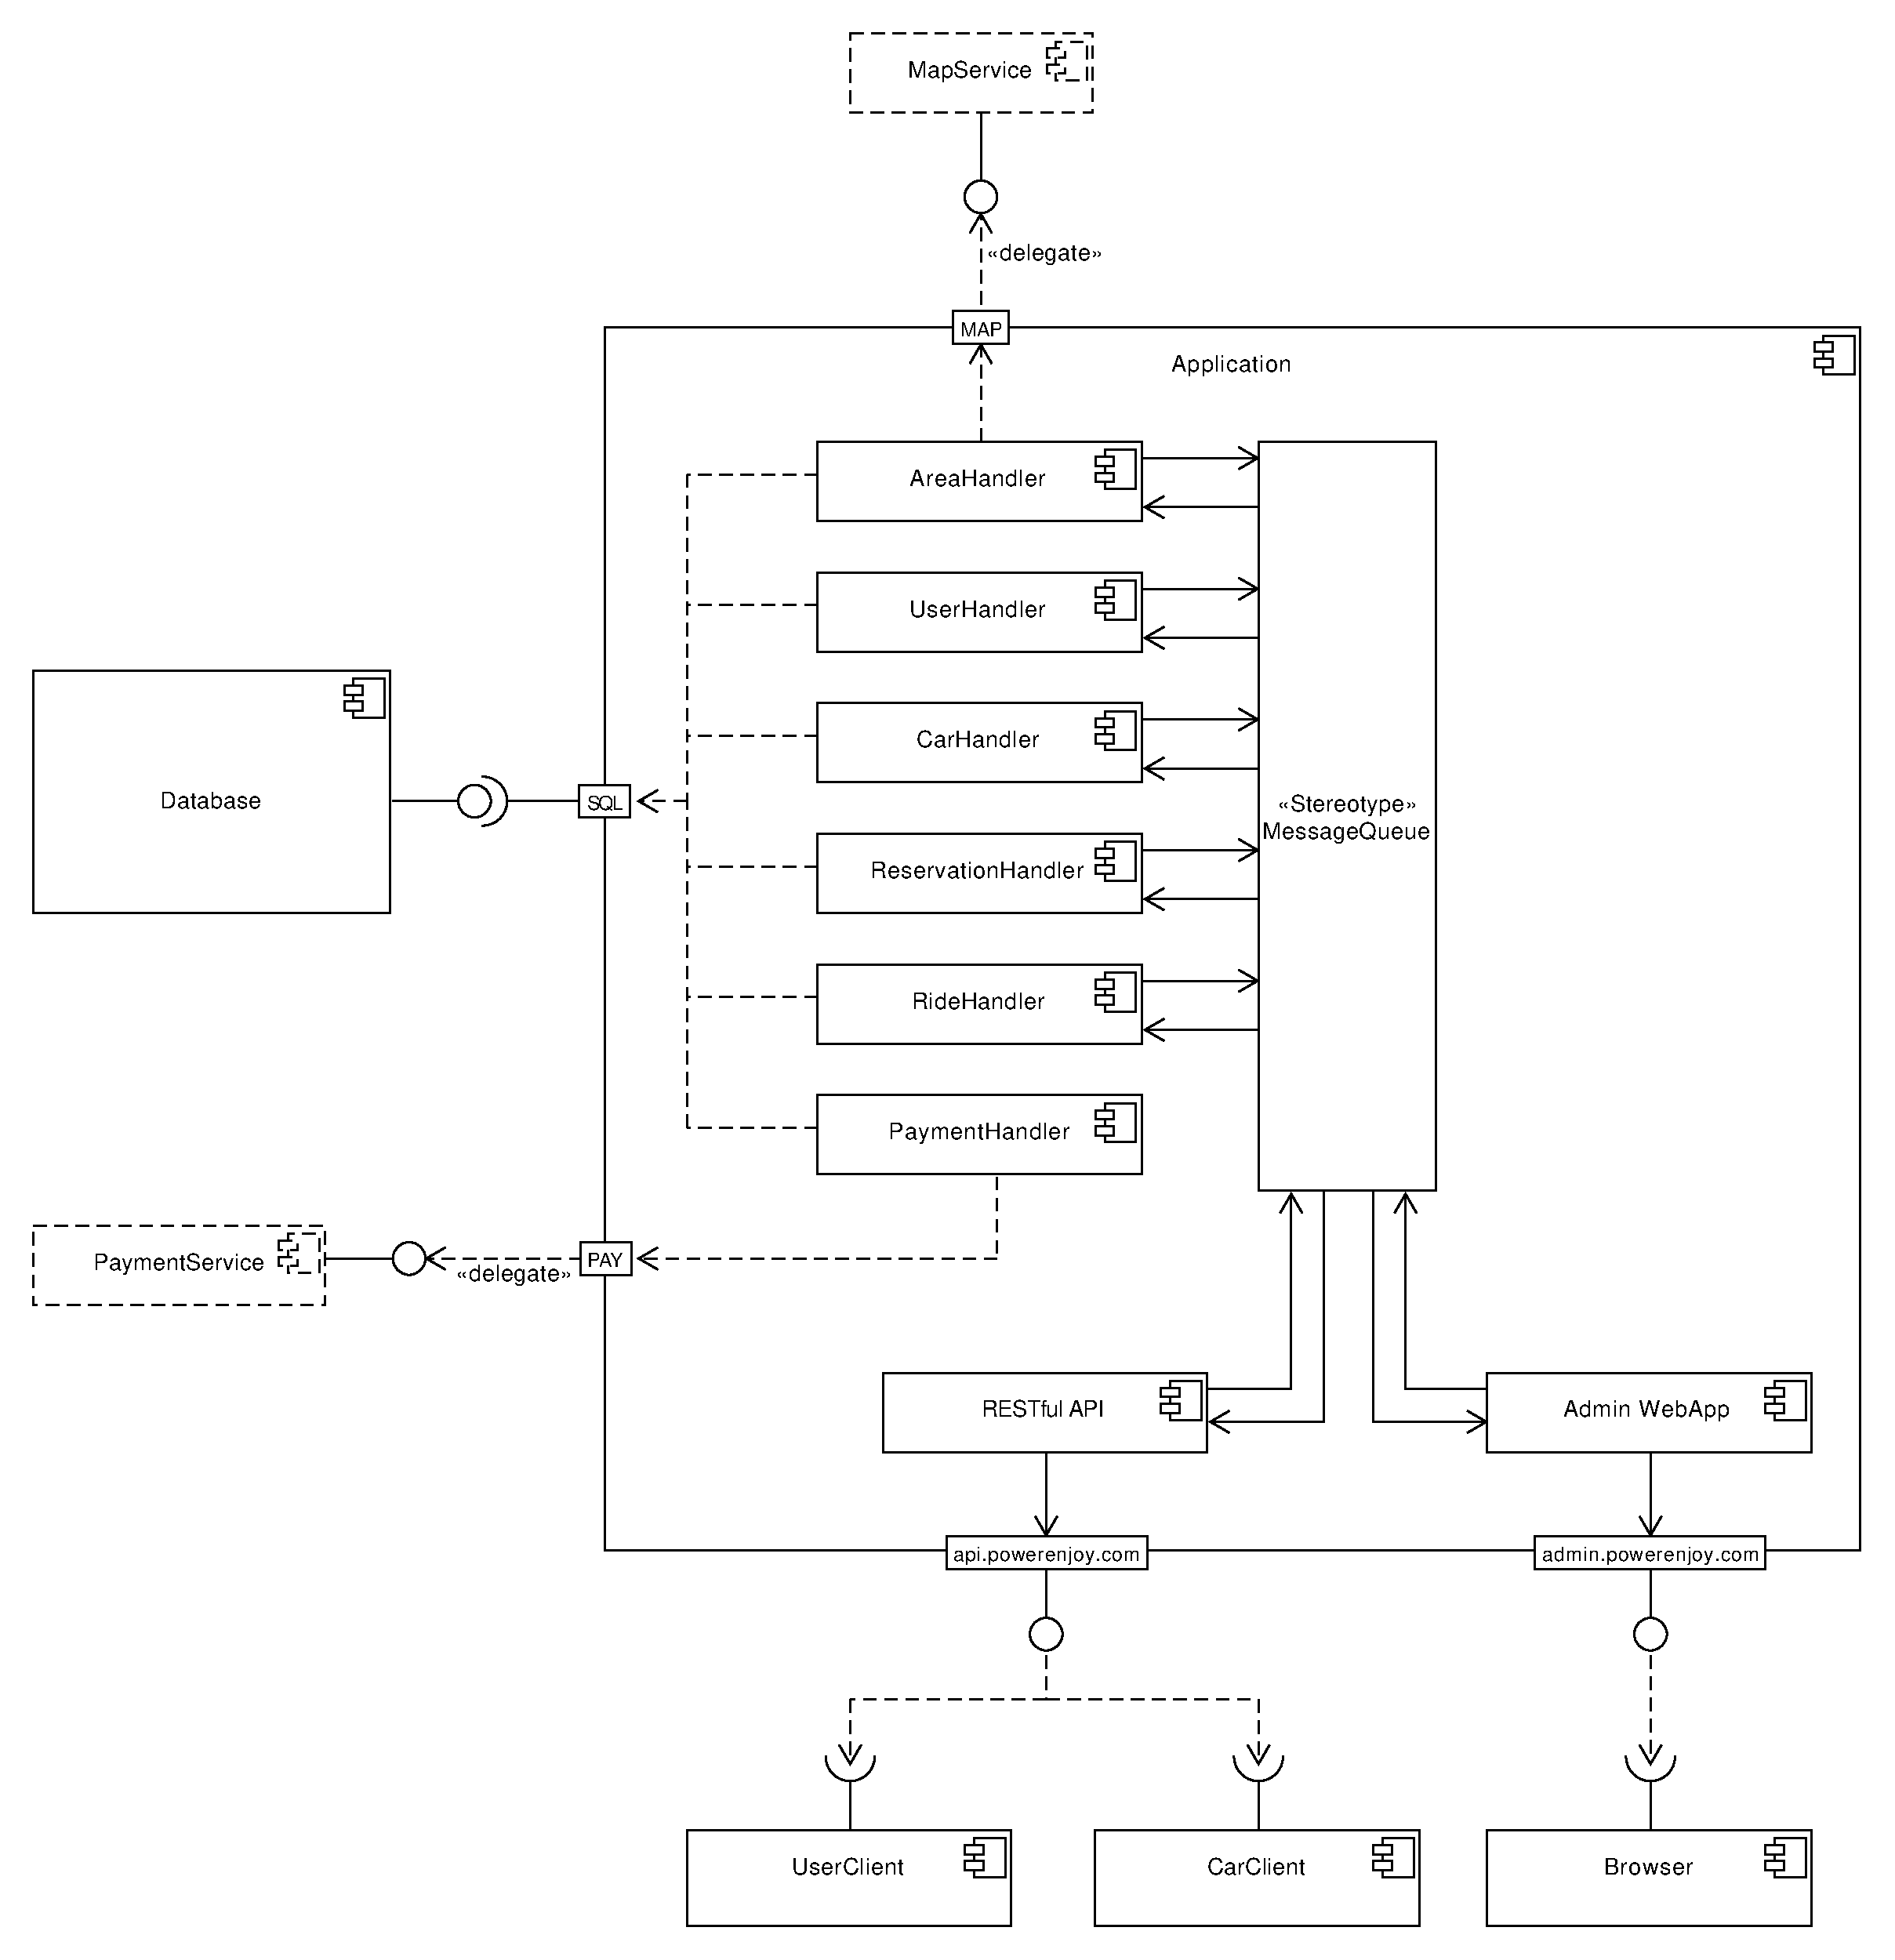
\includegraphics[width=\textwidth]{low_level_components}
\caption{Component view: Internal Low Level Architecture}
\label{fig:i_l_l_comp}
\end{sidewaysfigure}

\pagebreak
\subsubsection{Microservices}
\paragraph{Router}
The Router is the first of our internal component. The idea behind is that this is the component
delegated to do the initial parsing of the request coming from the client. It will analyze
the URI and the HTTP method following the REST principles and based on that informations,
it will produce a message to be enqueued. Once it will get back a reply from the service
corresponding to the initial request, it will send back that response to the client.

\paragraph{UserHandler}
This service deals with everything that concerns users. It's invoked to perform user creation
and to deal with requests coming from users devices. All the informations involving users
will be passed from the router to this component. In order to gather the required information
it may invokes other services as well.

\paragraph{CarHandler}
This is the car counterpart of what we have already discussed for users. This component will
register new cars when they are added to the system and provide informations about cars
position, charge status or availability.

\paragraph{ReservationHandler}
ReservationHandler provides informations related to reservations. It is likely that it will
respond to UserHandler messages when the list of reservations for a single user is requested.
Alternatively, CarHandler can retrieve a list of all reserved cars. 

\paragraph{RideHandler}
This is the component that handles all rides information. It can be queried in order to have
a list of all rides, of the active ones, rides belonging to a specific user
(they may be active or not) and is the link to payment and discount informations. All the informations
displayed on the car monitor during the ride are gathered from this service.

\paragraph{PaymentHandler}
The PaymentHandler has to main purposes. The first one is to manage the operations dealing
with the external Payment service. The second one is to save information about users payments
after it gets a reply from the external service. 
This is done in order to provide a history of all payments or a list of pending payments.


\paragraph{AreaHandler}
This component is in charge of operations dealing with all the safe areas belonging to the company.
Safe areas are stored to know exactly their position and the type of the safe area, being it
a normal area or a power grid station.

\pagebreak

\subsection{Deployment}
This section will be dedicated to the deployment strategy adopted for our application. Figure~\ref{fig:depl}
shows the physical structure of the system and we are going to describe it in greater detail.

\paragraph{IaaS} The infrastructure for our deployments will not be based on bare metal servers
but we preferred to adopt an approach based on IaaS. In this way we can benefit from the
flexibility provided by this kind of services that will allow us to start small and scale
up, when our user base will grow.  

\paragraph{Servers} We choose to use a three-tier architecture with three different servers:
\begin{itemize}
    \item{Reverse Proxy}: This our first tier and has the main role to redirect users request to
        the application server. Other jobs executed on this server are: caching, load balancing
        and serving static files.
        Load balancing is a function that maybe is not going to be exploited in the beginning,
        but we expect it to become useful, when the load of out application server will increase.

    \item{Application Server}: This is the server containing our application and is our second tier.
        All requests will be redirected here in order to provide a response. Looking at
        Figure~\ref{fig:depl}, this component is represented by a solid rectangle with additional
        dashed rectangles around it. This kind of notation represent our idea that in the
        beginning there will be only one application server but, when the load will increase,
        this is the first component that will be affected by it. For this reason we want to
        be able to add other instances of our application seamlessly. This is made possible
        thanks to our previous decisions to use IaaS and a load balancer, while data consistency
        will be granted by a stateless architecture and persistence delegated to the database.

    \item{Database Server}: Our third layer is the database. In this case we adopted a
        traditional approach and used a relational database. Since RDBMS are usually well
        optimized to work even under heavy load, we don't expect to need any kind of
        replication right now.

\end{itemize}
\begin{sidewaysfigure}
\centering
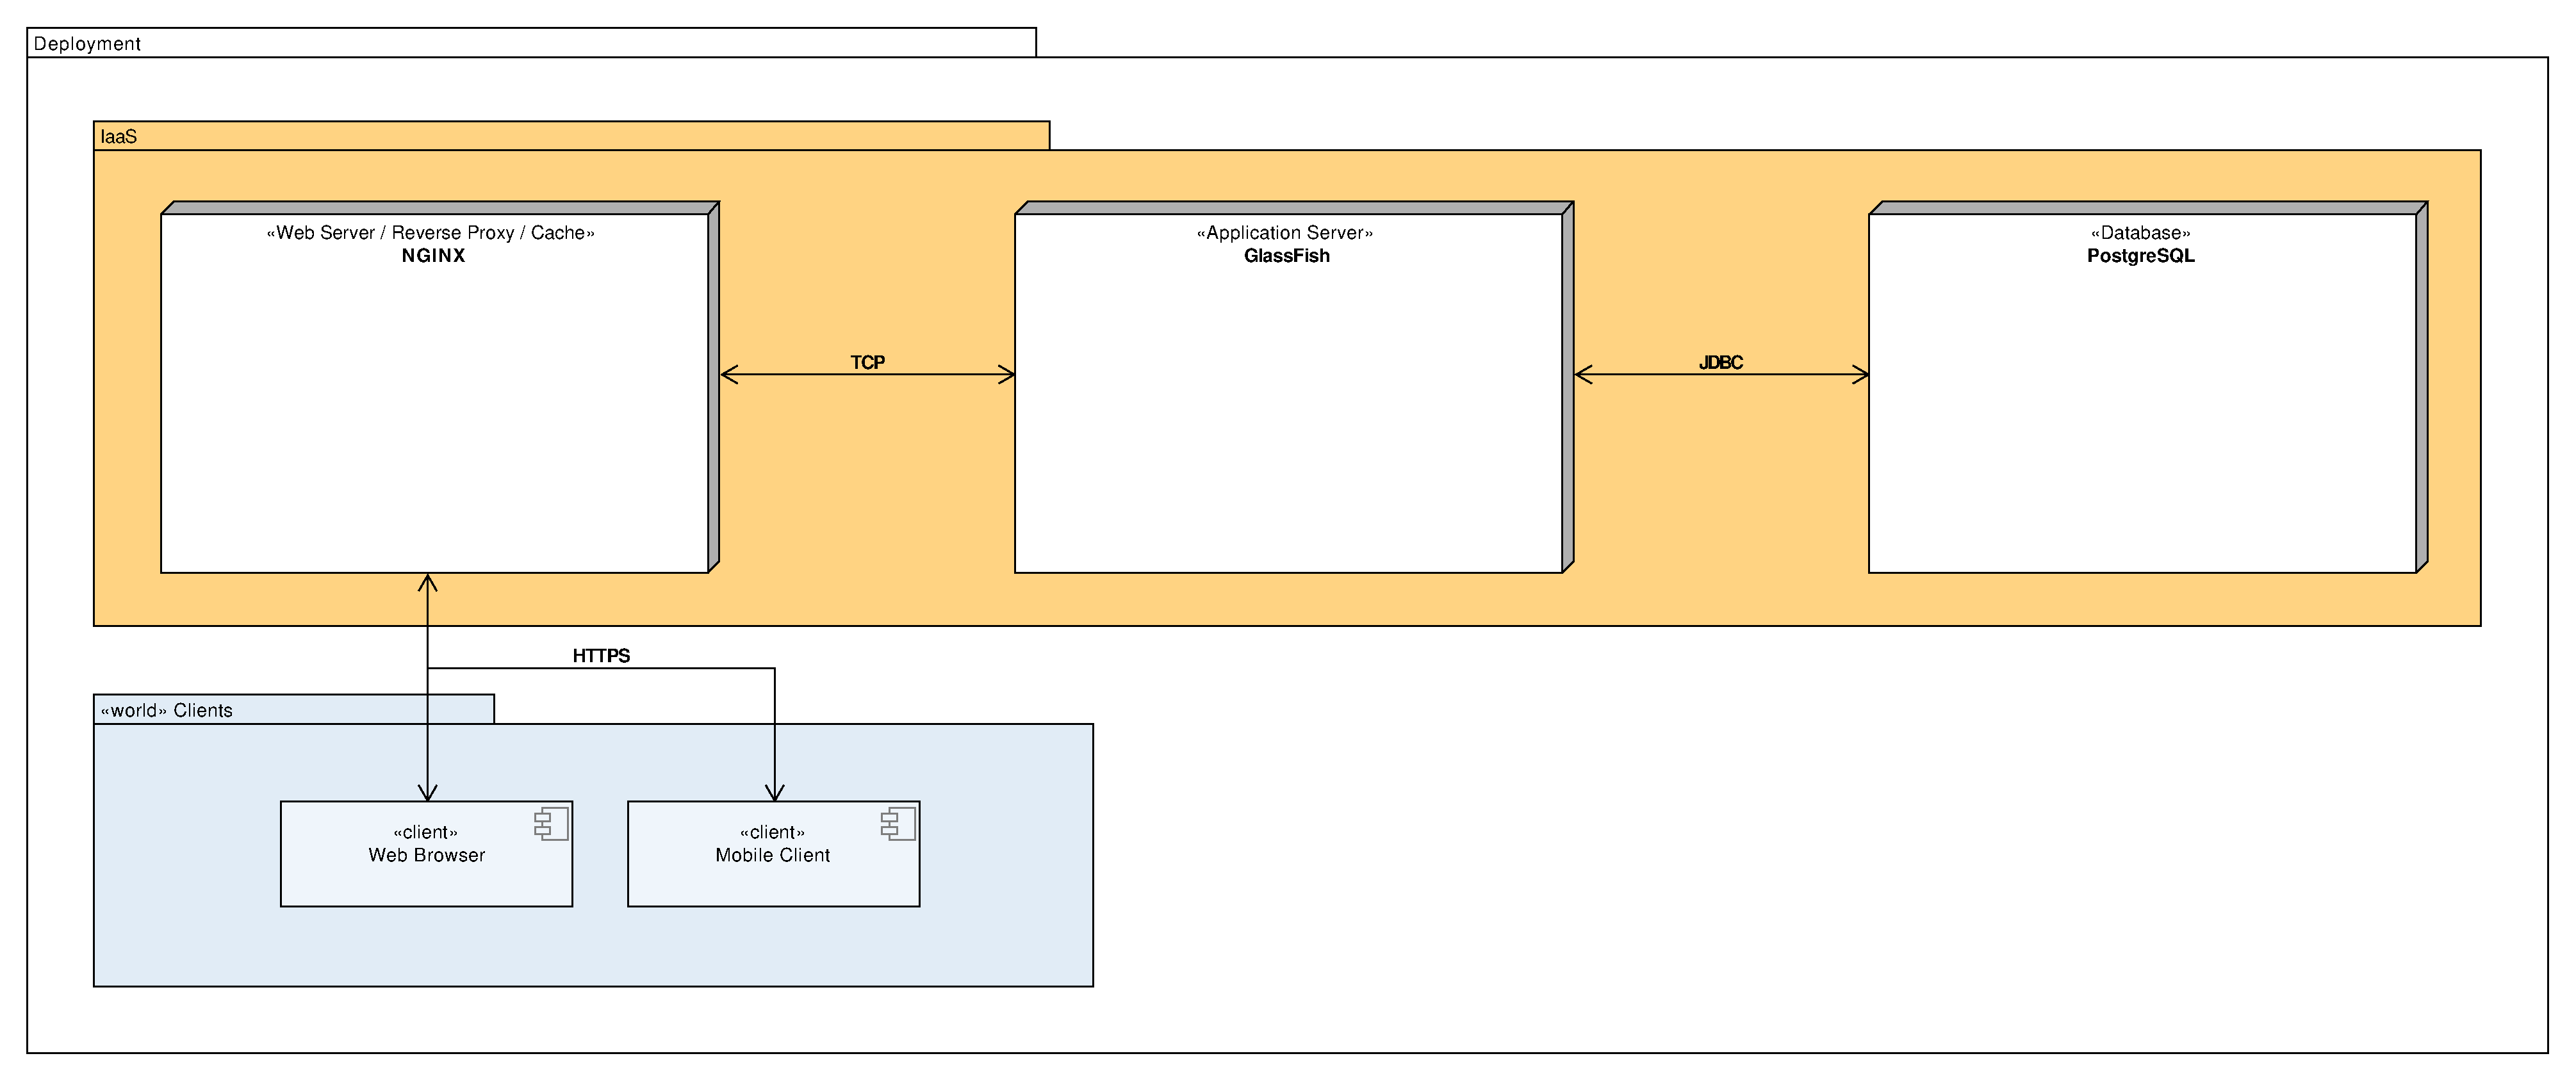
\includegraphics[width=\textwidth]{deployment}
\caption{Deployment view}
\label{fig:depl}
\end{sidewaysfigure}
